\documentclass[10pt]{beamer}
\usetheme{Berlin}
\usecolortheme{lily}
\usepackage[utf8x]{inputenc}
\usepackage[english]{babel}
\usepackage[T1]{fontenc}
\usepackage{lmodern}
\usepackage{amsmath}
\usepackage{amssymb}
\usepackage{enumerate}
\usepackage{graphicx}
\usepackage{cite}
\usepackage{listings}
\usepackage{hyperref}
\usepackage{lipsum}
\usepackage{tikz}
\beamertemplatenavigationsymbolsempty

%\usepackage{pgfpages}
%\setbeameroption{show notes}
%\setbeameroption{show notes on second screen=left}

\newcommand{\docauthor}{Axel Angel}
\newcommand{\doctitle}{Towards Distortion-Predictable Embedding of Neural Networks}
\newcommand{\docsubtitle}{Presentation}
\newcommand{\eg}{e.g.}
\newcommand{\reff}[1]{~\ref{#1}}
\setkeys{Gin}{width=1.0\textwidth}

\author{\docauthor}
\title{\doctitle \\ \docsubtitle}

\pdfinfo{
    /Author (\docauthor)
    /Title (\doctitle)
    /Subject (\docsubtitle)
    }

% FIXME: change color of subtitle
% FIXME: add epfl logo and teacher name

% fixme: more why = explain why
% FIXME: explain recap orally the goal: 1-2 sentences
% study of properties of CNN, embedding,
% predictable = control over embedding
% (before title)

\begin{document}
\begin{frame}
    \titlepage
\end{frame}

\note{\begin{itemize}
    % Summary (recap what said during presentation)
    \item present an example of application for our method
    \item brief recap of CNN
    \item found t-SNE is good for visualization
    \item not suitable for predictable embeddings
    \item generalized the contrastive loss
    \item provide comparisons in qualitative and quantitative forms
    \item several directions for future works
    \item final thoughts and conclude this work
\end{itemize}}

\begin{frame}
    \tableofcontents{}
\end{frame}

\section{Motivations}
\begin{frame}
    \frametitle{Motivations}
    \begin{itemize}
        \item Face recognition
        \item Develop the theory behind it
        \item Our work is a start
    \end{itemize}

    % FIXME: add figure (LeCun, face reco)
    % FIXME: what we want to do with face reco, not really clear
    % feed person picture into network, now abstract features, but want something more controllable, predictable (pose, expression, identity : separately)


    \note{\begin{itemize}
        \item there are examples of applications for our method.
        \item ``face recognition'': pose estimation, expression, mouth, identity
        \item benefit from predictable embeddings.
        \item face recognition is too hard to start
        \item we experimented with simpler datasets (with mnist and norb)
    \end{itemize}}
\end{frame}

\section{Review of CNNs}
\begin{frame}
    \frametitle{Review of CNNs}
    \begin{itemize}
        \item Architecture
        \item Similar to a blackbox
        \item We focus on the embedding
    \end{itemize}

    % fixme: show by hand neuron/layer
    % fixme: why conv works in images (less noise, pooling)
    % fixme: add CNN figure
    % fixme: maybe add adverserial image
    % fixme: define ``features'' = last layer output


    \note{\begin{itemize}
        \item architecture:
            \begin{itemize}
                \item built-in feature extractor (ConvNets)
                \item built-in classifier (NeuralNets)
                \item forward/backward SGD
            \end{itemize}

        \item unintuitive properties:
            \begin{itemize}
                \item adverserial attacks
                \item conditions of good convergence
                \item unpredictable embedding
            \end{itemize}
        \item this work focus predictability of embedding under transformations.
            % fixme: which transfo
        \item can make them learn certain properties
    \end{itemize}}
\end{frame}

\section{Visualization with t-SNE}
\begin{frame}
    \frametitle{Dimensionality Reduction with t-SNE}
    \begin{itemize}
        \item Definition of t-SNE % fixme: give acronym
        \item Optimized properties (spring model)
        \item Previous works
    \end{itemize}

    % fixme: state-of-the-art for dim reduc, why we use it
    % fixme: already applied on mnist


    \note{\begin{itemize}
        \item define t-SNE: reduce dataset from nD to 2D, with optimisation problem.
        \item original points are Gaussian, new points are Student distr.
        \item optimisation make the new repr matches the original: based on points distances
        \item how we did: train/test MNIST, behead last layers and reduce with t-SNE
        \item many papers showed this already but few worked on distortions
        \item kind of distortion: translations, rotations.
    \end{itemize}}
\end{frame}

% fixme: +1 slide to present on mnist without transfo (explain what we do)
% fixme: then say we add transfo

\begin{frame}
    \frametitle{Visualization with t-SNE}
    \begin{figure}[h]
        \begin{center}
            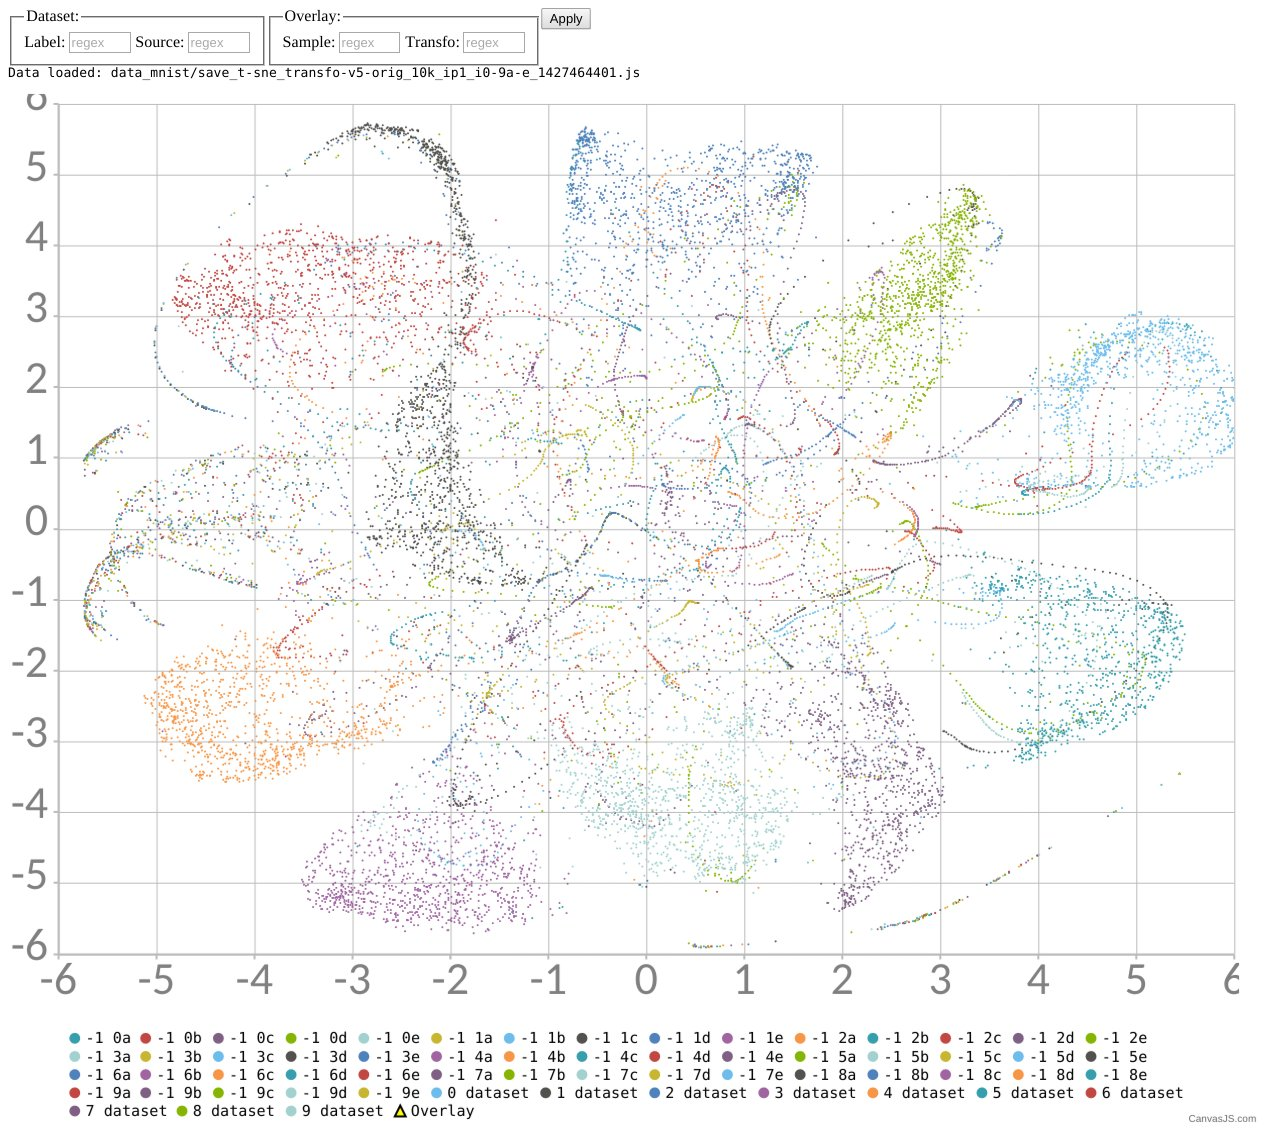
\includegraphics[width=0.5\textwidth]{../report/thesis_figures/mnist_nda_tsne2.jpg}
        \end{center}
    \end{figure}
    \begin{itemize}
        \item Results are unpredictable
        \item We could adapt t-SNE
    \end{itemize}
    However there exist better alternatives.

    % fixme: explain mnist
    % fixme: not really consistency


    \note{\begin{itemize}
        \item discontinuities, questionable clustering
            \begin{itemize}
                \item along some transfo, esp translation
                \item clusters are dominated by distortions (instead of digits)
                \item clusters are mixed up, unclear/confusing
            \end{itemize}
        \item limitations
            \begin{itemize}
                \item lack of control (opti problem is unlabeled)
                \item cannot add points, recompute from scratch, costly
            \end{itemize}
        \item fails to provide concluding results
        \item could reformulate/adapt t-SNE but better alternative exists
        \item what we show in the following
    \end{itemize}}
\end{frame}

\section{Towards Predictable Embeddings}
\begin{frame}
    % explain concepts
    \frametitle{Dimensionality Reduction with NN}
    Learn pair relations directly, by using:
    \begin{itemize}
        \item DrLIM (…) % fixme
            % fixme: instead of training NN for classification, use for dim redu with certain property
            % properties are …
        \item Neural networks (CNN or NN)
        \item Siamese architecture % fixme: << figure
        \item Contrastive loss
            \begin{eqnarray}
                L = \frac{1}{2} Y (D_W)^2 + \frac{1}{2} (1-Y) \max(0, m - D_W)^2
            \end{eqnarray}
    \end{itemize}
    %many pairing relations can be learned directly into embeddings.

    % fixme: explicit: it's DrLIM, not t-SNE, it's NN mapping, no projection, detail properties of this plot
    \begin{figure}[h]
        \begin{center}
            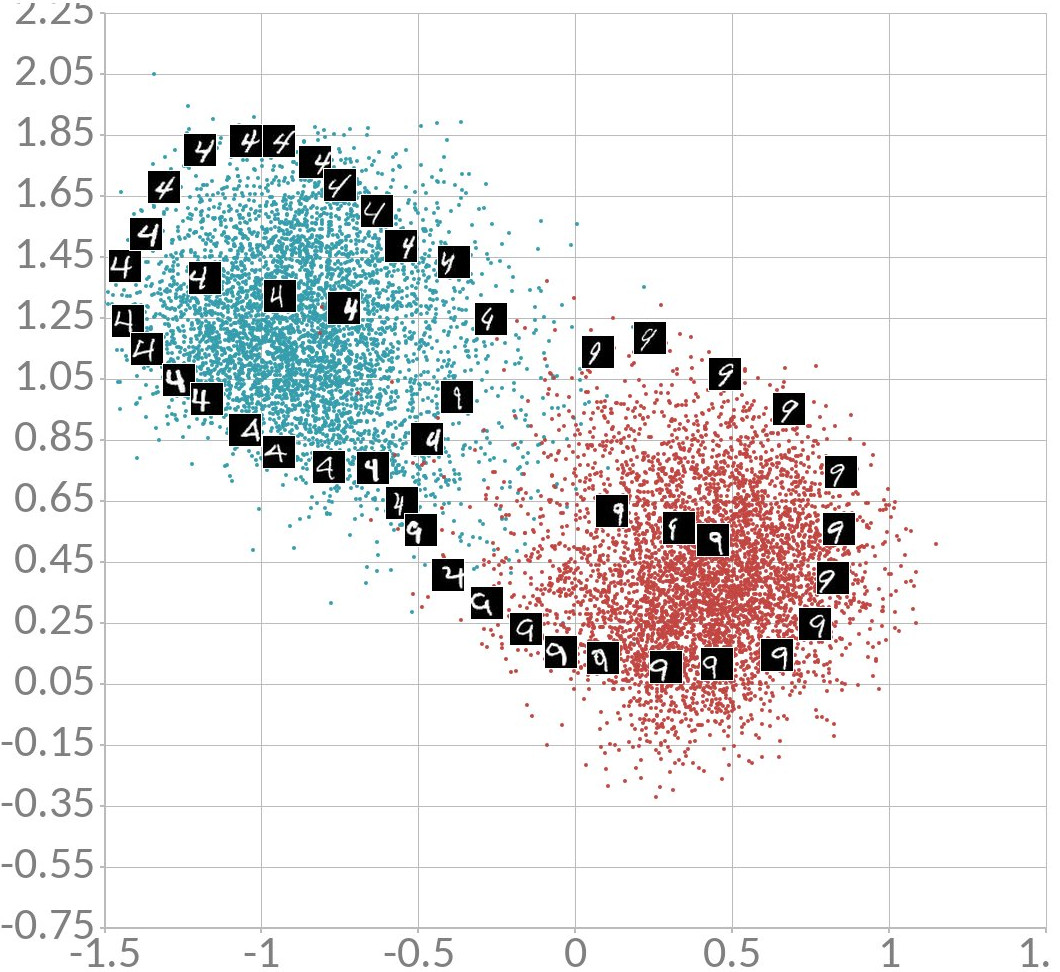
\includegraphics[width=0.45\textwidth]{../report/thesis_figures/mnist_cl_drlim.jpg}
        \end{center}
    \end{figure}


    \note{\begin{itemize}
        \item neural networks can express complex non-linear mappings
        \item learn relation: mapping of pairs (2 images) to 1/0 similarity
        \item previous work {\em Dimensionality Reduction by learning an invariant mapping} (DrLIM) by: Raia Hadsell, Sumit Chopra, Yann LeCun
        \item showed: neural networks can learn structured embeddings
        \item showed: can be used for dimensionality reducing
        \item training with: siamese and contrastive for loss (also used for face recognition, same authors)
        \item trained networks to represent: MNIST by similarity in 2D, camera viewpoint in 3D
        \item points similar = close together, similar to t-SNE
    \end{itemize}}
\end{frame}

\begin{frame}
    \frametitle{Predictable Embeddings}
    % fixme: first why we extend (we want predictable), why would it work (because more control, constraint component/dimensions correspond to relation)
    In our work we present:
    \begin{itemize}
        \item An extension of this loss for $N$ relations
            % fixme: change color the sum
            \begin{eqnarray}
                L = \frac{1}{2} \sum_{i=1}^p \left( Y_i (D_{Wi})^2 + (1-Y_i) \max(0, m_i - D_{Wi})^2 \right)
            \end{eqnarray}
        \item Qualitative and quantitative results
    \end{itemize}


    \note{\begin{itemize}
        \item our work is based on the mentioned paper
        \item we reuse the same concepts but extend contrastive loss
        \item our goal is: learn more similarities, separately, add more control
        \item can decide which dimensions express what similarity (align to axes)
        \item plots serve as qualitative results for human to visually compare
        \item but we also introduce quantitative measures to compare with previous work (reproduce DrLIM work)
    \end{itemize}}
\end{frame}

\begin{frame}
    \frametitle{Results On MNIST}
    \begin{itemize}
        \item Multiple relations at once
    \end{itemize}

    % fixme: this is same space, two projections
    % fixme: left one looks the same but we add the right

    \begin{figure}[h]
        \begin{center}
            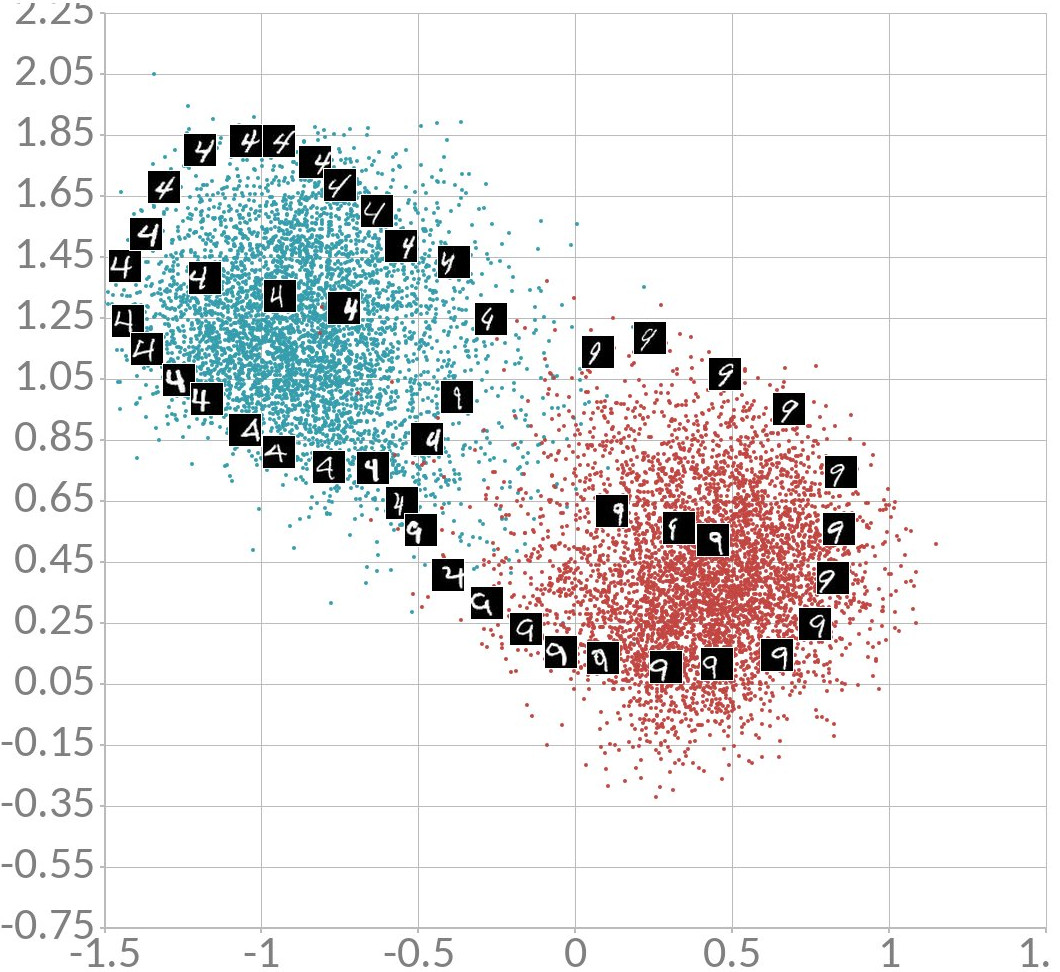
\includegraphics[width=0.45\textwidth]{../report/thesis_figures/mnist_cl_drlim.jpg}
            \vspace{1cm}
            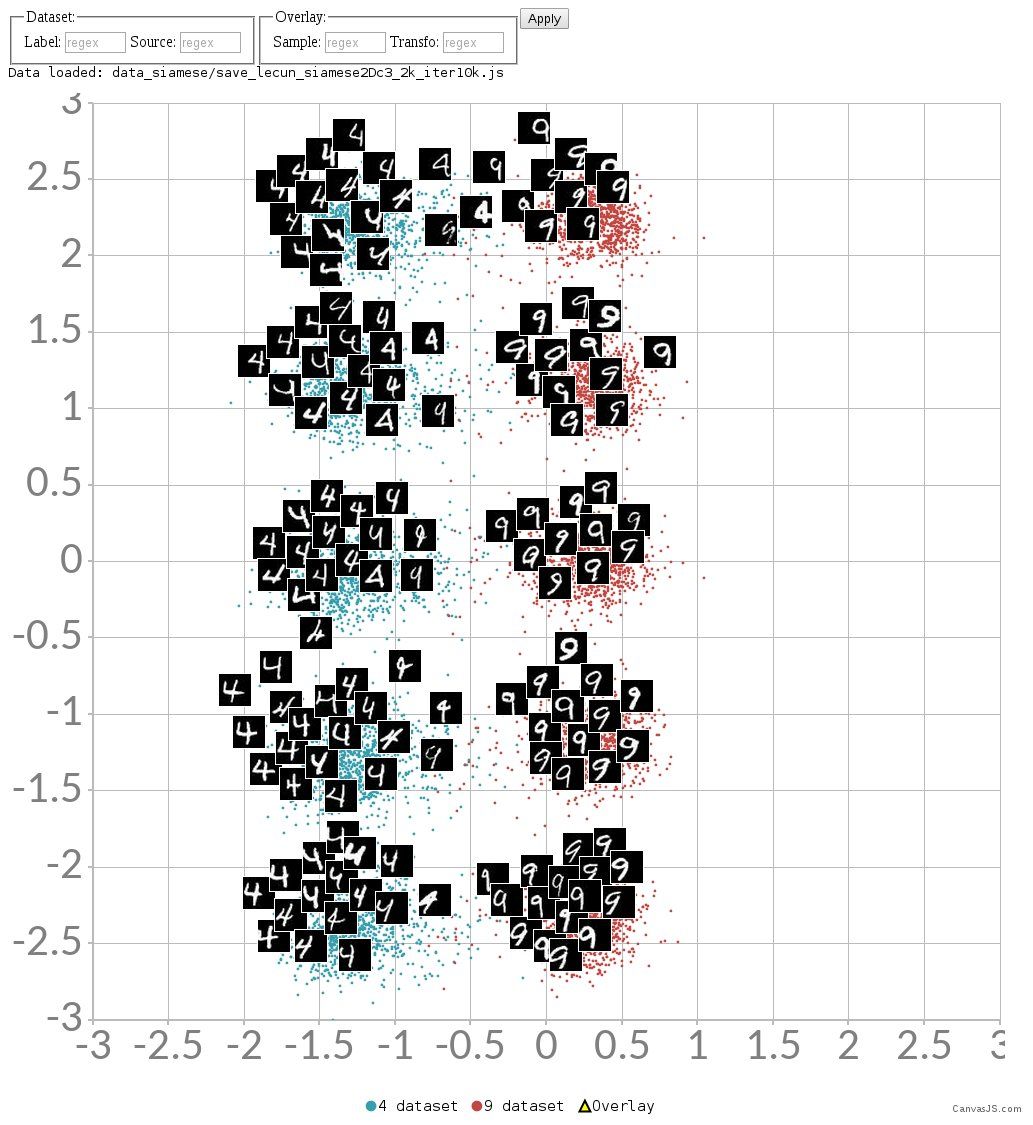
\includegraphics[width=0.45\textwidth]{../report/thesis_figures/mnist_cl2d2.jpg}
        \end{center}
    \end{figure}


    \note{\begin{itemize}
        \item quick recap dataset MNIST
        \item on this experiment MNIST, we train with two classes like DrLIM
        \item learn to put similar numbers together
        \item DrLIM do it in 2D, we do the same but add a new dimension
        \item it serves to express translations without disturbing the other 2D
        \item models can learn >1 relations: correctly (quality) and effectively (1 model)
        \item quality: qualitative measures (in 2D) show it's as good and we cannot tell them apart (good coherence inside clusters)
        \item effectively: 1 model = train 1 model, share weights/features for both tasks
        \item we also tried on non-linear transfo (rotations) with same results (similar clustering).
    \end{itemize}}
\end{frame}

% fixme: add slide for common loss

\begin{frame}
    \frametitle{Results On NORB}
    \begin{itemize}
        \item More predictable structures
    \end{itemize}


    % fixme: separate this slice: * show ours two viewpoints * briefly compare DrLIM and our (same viewpoint)
    \begin{figure}[h]
        \begin{center}
            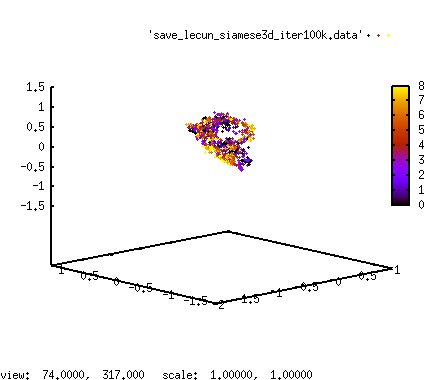
\includegraphics[width=0.45\textwidth]{../report/thesis_figures/norb_drlim1.jpg}
            % fixme: zoom shape inside figure
            \vspace{1cm}
            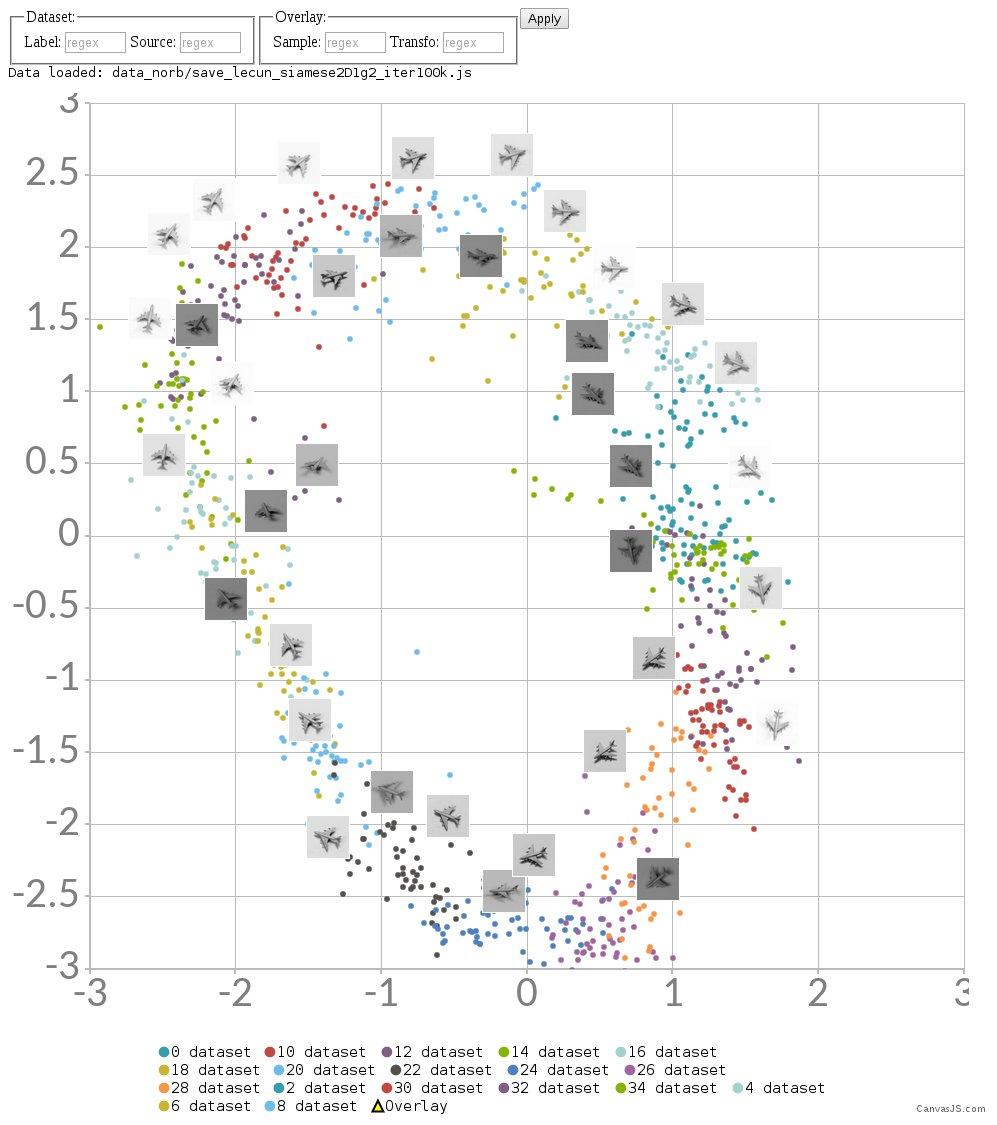
\includegraphics[width=0.45\textwidth]{../report/thesis_figures/norb_cl2d.jpg}
        \end{center}
    \end{figure}


    \note{\begin{itemize}
        \item quick recap dataset NORB
        \item on this experiment NORB, same task DrLIM
        \item found our solution easier to work with (converge to correct shape)
        \item cylinder: cyclic structure for azimuth, ordered value for elevation
        \item major difference: alignment with axes, points are more separated.
        \item quality seems better (wider radius, more separated) but our quantitative measure doesn't show that
    \end{itemize}}
\end{frame}

% fixme: add slide for common loss (we proposed quantitaive measures)
% what we choose, why (was not done before)

\section{Conclusion}
\begin{frame}
    \frametitle{Future Work}
    \begin{itemize}
        \item Make experimental comparisons with regression
        \item Show predictability with auxiliary networks
        \item Fields applications: Face Recognition, Bio-Medical Imaging.
    \end{itemize}

    \note{\begin{itemize}
        \item models can learn multiple pairing at once: MNIST (similarity + class + transfo), NORB (azimuth + elevation)
        \item like regression but major differences (abs/relative pos + hard/soft margins); absolute position is not easily defined in applications like face reco where (eg face expression: smile, sad, chose value? Let the model find what's good); future work should compare our solution to regression on MNIST (more constraints help?)
        \item direct predictability, train a model to predict other-transfo features given one-transfo features (ex: transl 0 -> trans N for all N); the auxiliary network learn to map features of a particular transfo to all other transfo (accuracy = measure of pred)
        \item future work can show how our solution works with fields ; like face reco (multiple face features: pose, expression, mouth, eyes, eyebrows, …); like bio medical (instead of all costly rotation of 3D images -> features, compute directly independent features with its rotation).
    \end{itemize}}
\end{frame}

% like summary
\begin{frame}
    \frametitle{Conclusion}
    \begin{itemize}
        \item Motivations of our work
        \item Unexpected results using t-SNE
        \item Proposition of an alternative with NN
        \item Further directions are promising
    \end{itemize}

    \note{\begin{itemize}
        \item began motivation with applications (face reco, bio imaging)
        \item small overview NN (their unintuitive properties, black box)
        \item we explore one particular aspect: embeddings predictability
        \item first try with t-SNE unexpected results, too many limitations
        \item we decided go to pure NN solutions (aspects of data directly into embedding)
        \item previous work already proposed solutions for 1 relation
        \item we wanted: more information to be encode and making sure we have a more predictable result by adding more constraints on dimensions
        \item we extended the contrastive loss to allocate dimensions per relation (more control, share weights, efficient)
        \item our good results demonstrated the practicality of our solution on two datasets
        \item however our work is only a beginning: measures should be defined to capture predictability and experiments should try our solution on practical applications.
    \end{itemize}}
\end{frame}

% fixme: append slides: t-sne formula

\end{document}
